\documentclass[conference,10pt]{IEEEtran}
\IEEEoverridecommandlockouts
% The preceding line is only needed to identify funding in the first footnote. If that is unneeded, please comment it out.
\usepackage{cite}
\usepackage{ctex}
\usepackage{amsmath,amssymb,amsfonts}
\usepackage{algorithmic}
\usepackage{graphicx}
\usepackage{textcomp}
\usepackage{xcolor}
\usepackage{float}
\usepackage{subfigure}
\usepackage{hyperref}

\hypersetup{hidelinks,
					colorlinks=true,
					allcolors=blue,
					pdfstartview=Fit,
					breaklinks=true}
% \usepackage{hyperref}
\def\BibTeX{{\rm B\kern-.05em{\sc i\kern-.025em b}\kern-.08em
    T\kern-.1667em\lower.7ex\hbox{E}\kern-.125emX}}
\begin{document}

\title{Homework1:倒立摆实验报告\\}

\author{\IEEEauthorblockN{
    % 1\textsuperscript{st} 
承子杰}
\IEEEauthorblockA{\textit{dept. AMSS(数学与系统科学研究院)} \\
\textit{of CAS (中国科学院)}\\
%chengzijie22@mails.ucas.ac.cn\\
202228000243001}}

\maketitle

\begin{abstract}
倒立摆系统控制是一个经典的强化学习问题,我们使用欧拉法对其连续动力学模型进行离散建模,创建仿真环境。对于问题求解我们分别尝试使用基于价值策略的强化学习算法和基于策略梯度的强化学习算法。对于价值函数逼近,我们分别尝试基于离散价值空间和逼近器进行刻画,对于价值函数更新,我们使用基于全局的DQI算法和基于采样的Sarsa算法与Q-Learning算法,策略梯度方面主要尝试了REINFORCE算法与Actor-Critic算法。最后我们通过实验结果对问题和算法进行了一个简单总结。
\end{abstract}
\section{简介}
倒立摆是将一个物体固定在一个圆盘的非中心点位置, 由直流电机驱动将其在垂直平面内进行旋转控制的系统(见图\ref{pic1})。 由于输入电压是受限的, 因此电机并不能提供足够的动力直接将摆杆推完一圈。相反, 需要物体来回摆动收集足够的能量。倒立摆问题的目标是将物体推起到最高点并使其稳定在该位置。

\begin{figure}[H]
    \centering
    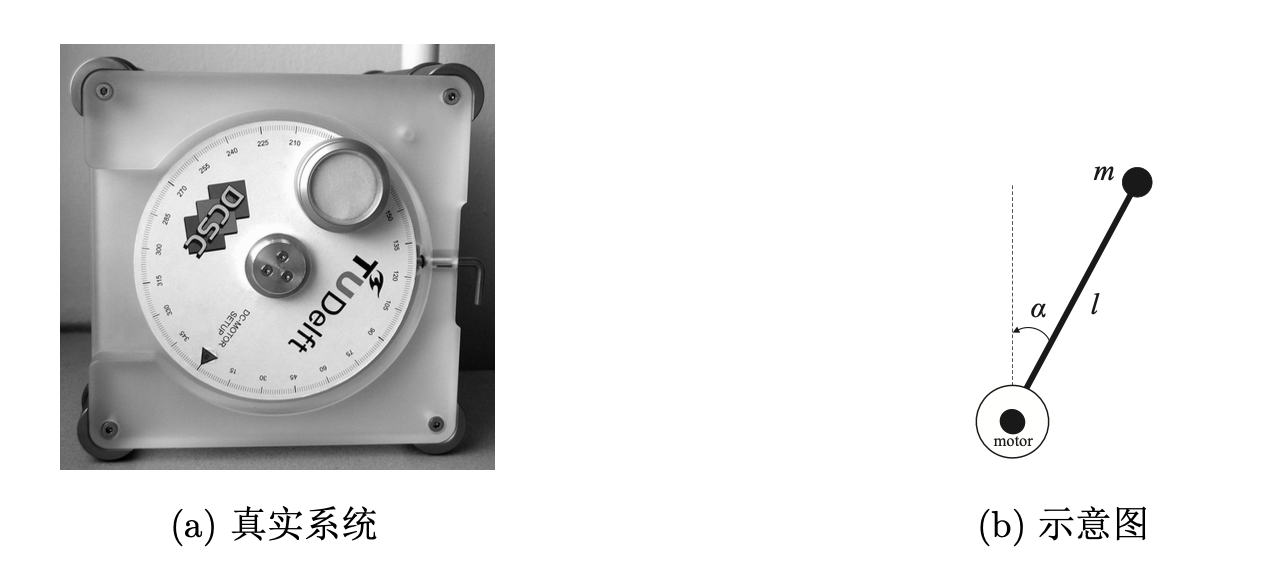
\includegraphics[scale=0.25]{./figure/pic1.png}
    \caption{倒立摆示意图}
    \label{pic1}
\end{figure}

根据欧拉法,我们可以将倒立摆系统的连续时间动力学模型进行离散化,从而建立仿真模拟环境。观察其离散动力学方程,我们可以发现,倒立摆每一时刻状态的变化(角度位置)受角速度变量影响,而通过改变直流电压,我们可以干预角加速度的变化,进而影响角速度的走向。

因此,通过对角度和角速度空间进行等距离划分,对直流电压进行特征动作选择和奖励函数设置,我们可以将倒立摆问题的求解转化为一般形式下的有限马尔可夫决策过程(MDP)。根据价值迭代和策略迭代的思想,可以利用离散Q价值迭代算法,对问题进行求解。鉴于对全状态空间搜索计算量的考量,可以使用基于采样的 Sarsa算法、Sarsa$(\lambda)$算法和 Q 学习算法。另一方面,Q函数逼近依赖于离散空间的划分细度,鉴于维数方面的考量,我们可以使用 RBF 核函数构建特征向量,使用线性逼近器获得 Q 函数的连续化逼近。由于浅层神经网络可以拟合任意可微函数,且不需要人工构造特征向量,因此使用DQN算法是更佳的选择。

另一方面,我们可以抛开Q价值函数,直接对最优动作策略进行拟合。我们尝试使用了REINFORCE算法与Actor-Critic算法对问题进行求解。结果表明,动作策略均收敛于局部最优解,并未成功实现最优控制。此外,基于策略函数建模存在方差较大,训练不稳定等结果,对于倒立摆问题似乎并不适合。

经过实验,大部分算法都获得了问题的预期求解,但最优动作的选择并不尽相同。通过对各算法训练中表现的分析,我们在总结中对倒立摆问题进一步讨论。
\section{倒立摆系统}
\subsection{符号说明}
\begin{table}[H]
	\centering
	\caption{倒立摆系统参数变量}
	\label{tb1}
	\begin{tabular}{llll}
		\hline
		变量&取值  &单位  &含义   \\ \hline
		\textit{m}& 0.055 & kg & 质量 \\ 
		\textit{g} & 9.81 & $\mathrm{m}/\mathrm{s}^2$ & 重力加速度  \\ 
		\textit{l} & 0.042 & m & 重心到转子的距离 \\ 
		\textit{J}&$1.91\cdot10^{-4}$  & $\mathrm{kg}\cdot\mathrm{m}^2$ &转动惯量  \\ 
		\textit{b}&$3\cdot10^{-6}$  &$\mathrm{Nm\cdot s/rad}$  & 粘滞阻尼 \\ 
		\textit{K}& 0.0536 & Nm/A & 转矩常数 \\
		\text{R}& 9.5 & $\Omega$ &转子电阻  \\
		$T_s$&0.005&s&动作采样时间\\
		$a$ & $[-\pi,\pi)$ &  rad & 角度  \\
		$\dot{a}$& $[-15\pi, 15\pi]$ & rad/s & 角速度  \\
		$\ddot{a}$& - & $\mathrm{rad/s^2}$ &   角加速度\\ 
		$u$&[-3,3]&V&直流电机电压\\
		$\gamma$&-&-&折扣因子\\
		$s$&-&-&状态\\ \hline
	\end{tabular}
\end{table}
\subsection{物理学分析与仿真环境}
根据物理学模型,倒立摆系统连续时间动力学模型满足方程\ref{eq1}
\begin{equation}
\ddot{a} = \dfrac{1}{J}\large\left(mgl\sin(a)-b\dot{a}-\dfrac{K^2}{R}\dot{a}+\dfrac{K}{R}u\large\right)
\label{eq1}
\end{equation}
使用欧拉法,我们可以获得离散动力学模型(式\ref{eq2})
\begin{equation}
	\left\{
	\begin{array}{l}
		a_{k+1}=a_k+T_s\dot{a}_k\\
		\dot{a}_{k+1}=\dot{a}_k+T_s\ddot{a}(a_k,\dot{a}_k, u)\\
	\end{array}\right.
\label{eq2}
\end{equation}
各方程中参数的含义与取值由表 \ref{tb1} 给出。

通过分析物理学方程,系统状态包含摆杆的角度和角速度, 即 $s=[a,\dot{a}]^T$。角度 $a$ 取值范围在 $[-\pi, \pi]$rad 之间,其中 $a=-\pi$ 表示摆杆垂直指向下, $a=0$ 表示摆杆垂直指向上。某一状态的角度取值若超出给定范围,则对应加上或减去 $2\pi$ 进行规范化。角速度限制在$[-15\pi,15\pi]\mathrm{rad/s^2}$ 内,对于超出的角速度我们进行相应的截断处理。系统可以采取的动作为直流电机的电压,动作范围限制在 $[-3, 3] \mathrm{V}$ 之内。

系统的初始状态为 $s=[-pi,0]^T$,即摆杆静止垂直指向下,控制的目标是摆杆摆起且稳定在最高点,即 $s=[0,0]^T$。运动过程的每一状态下,我们对目标角度偏差和角速度进行相应惩罚。由于我们更倾向于系统采取小电压,使摆杆的动作变化连续稳定,因此我们对电压也进行一定的惩罚。因此,系统奖励函数定义为
\begin{equation}
	R(s,u) = -s^T\begin{bmatrix}
		5&0\\
		0&0.1\\
	\end{bmatrix}s-1\cdot u^2
\end{equation}
为了提高目标点附近奖励在初始时刻状态价值的重要性,我们选取折扣因子 $\gamma = 0.98$,这样最优策略能够以成功将摆杆摆起并稳定作为最终目标。

\section{基于价值函数的强化学习方法}
通过离散动力学建模,倒立摆系统控制问题已经转化为典型的马尔可夫决策过程。最直接的想法是使用广义策略迭代,即通过Q价值函数的评估提取贪心策略,再根据获得的策略改进Q价值函数。但对于倒立摆系统,存在两个问题:第一个问题是动作空间并非离散,在提取贪心策略时,我们无法有效的获得每一状态下的最优动作。解决这个问题最直接的方法是选择离散特征动作,通过计算对应特征下各离散特征动作的Q值,选取最优动作。另一个问题是Q函数的表示问题,对应解决的方法有状态空间离散化表示与使用逼近器逼近表示。
\subsection{离散化方法}
解决Q函数表示最直接的方法是将状态空间离散。对每一个离散状态,我们使用一个常数来表示其Q值。通过状态空间离散,倒立摆系统直接转化为离散的马尔可夫决策过程,则常用的解决算法有动态规划(DP)、Sarsa、Q-Learning等。

\subsubsection{离散Q价值迭代(DP)}

离散 Q 价值迭代本质为动态规划方法,其基本的算法框架如下:
\begin{center}
	\fcolorbox{black}{gray!10}{\parbox{.9\linewidth}{
		1. 将状态空间离散化成状态子集 $\{S_k\},k = 1,...,K$ \\
		2. 定义有限动作集 $\{A_l\},l = 1,...,L$\\
	    3. 初始化$Q_{k,l}^{(0)} (e.g. Q_{k,l}^{(0)}  =0),i=0$\\
        4. repeat \{在第$ i $次迭代\}\\
    	5. $\quad$ 更新Q值$$Q_{k,l}^{(i+1)} = R_{k,l}+\gamma\max\limits_{l'}Q_{k',l'}^{(i)}$$
    	6. $\quad$ $i=i+1$\\
    	7. until $\Vert Q^{(i)}-Q^{(i-1)}\Vert\le\epsilon$
    }}
\end{center}
使用离散Q价值迭代算法主要存在如下几个问题:
\begin{itemize}
	\item 维数灾。随着状态空间维数的增加,算法的计算复杂度急剧上升,效率低下。
	\item Q 函数逼近的精确程度直接取决于状态空间分割的细度,对于变化比较细致的Q函数往往需要非常细致的分割。
\end{itemize}

\subsubsection{Sarsa}:针对离散Q价值迭代存在的第一个问题,我们可以使用采样的方法进行解决,Sarsa 就是一个不错的选择。其基本的算法框架如下:
\begin{center}
	\fcolorbox{black}{gray!10}{\parbox{.9\linewidth}{
			1. 将状态空间离散化成状态子集 $\{S_k\},k = 1,...,K$ \\
			2. 定义有限动作集 $\{A_l\},l = 1,...,L$\\
			3. 初始化$Q(s,a),\pi=\epsilon-greedy(Q),t=0$,初始状态$s_t=s_0$\\
			4. 采样动作 $a_t \sim \pi(s_t)$\\
			5. loop\\
			6.$\quad$ 执行动作$a_t$ 后获得观测量 $(r_{t+1} , s_{t+1})$\\
			7.$\quad$ 采样动作 $a_{t+1} \sim\pi(s_{t+1})$\\
			8.$\quad$  根据$ (s_t, a_t, r_{t+1}, s_{t+1}, a_{t+1}) $更新 Q
			$$Q(s_t, a_t) += \alpha(r_{t+1} + \gamma Q(s_{t+1}, a_{t+1}) − Q(s_t, a_t))$$
			9.$\quad$ 策略更新$$\pi=\epsilon-greedy(Q)$$
			10.$\quad$ $t+=1$\\
			11.end loop
	}}
\end{center}
此外我们可以引入资格迹进行权重衰减,从而使用整条轨迹上的状态-动作来强化Q函数。使用Sarsa算法存在的主要问题除了离散Q价值迭代中的第二个问题,还存在动作策略为$\epsilon-$ 贪心策略,并非完全贪心策略,系统在控制时有一定概率选择探索动作,而有时探索动作会对整个环境产生巨大影响。

\subsubsection{Q-Learning}
为了获得确定的动作策略,我们可以考虑使用基于离策略(off-policy)的 Q-learning。算法的基本框架如下:
\begin{center}
	\fcolorbox{black}{gray!10}{\parbox{.9\linewidth}{
			1. 将状态空间离散化成状态子集 $\{S_k\},k = 1,...,K$ \\
			2. 定义有限动作集 $\{A_l\},l = 1,...,L$\\
			3. 初始化$Q(s,a),t=0$,初始状态$s_t=s_0$\\
			4. 定义策略 $\pi_b = \epsilon-greedy(Q)$\\
			5. loop\\
			6.$\quad$ 执行动作$a_t\sim\pi_b(s_t)$ 并执行\\
			7.$\quad$ 获得观测量 $r_{t+1} , s_{t+1}$\\
			8.$\quad$  根据$ (s_t, a_t, r_{t+1}, s_{t+1})$更新 Q
			$$Q(s_t, a_t) += \alpha(r_{t+1} + \gamma \max\limits_{a'}Q(s_{t+1}, a') − Q(s_t, a_t))$$
			9.$\quad$ 策略更新$$\pi_b=\epsilon-greedy(Q)$$
			10.$\quad$ $t+=1$\\
			11.end loop
	}}
\end{center}
通过算法框架可以发现,Sarsa算法和Q-learning算法均使用时间序列差分误差来更新Q函数。但是Sarsa算法基于的是广义策略迭代的思想,Q-learning基于的是价值迭代的思想。
\subsection{逼近器方法}
使用离散化状态空间来表示Q函数存在一个相同的问题,即表示的精确度依赖于状态空间的分割细度。对于变化非常细微的Q函数,我们需要将状态空间分割的非常细致,从而导致状态空间维度过高,训练效率低下的问题。为此我们可以考虑使用逼近器。

构造线性函数是最为直接简单的逼近器,通过人工建立基于状态的特征向量表示,使用最小二乘等方法获得权重,即可以得到连续的Q函数表示。线性逼近器的表示能力往往依赖于特征向量,常见的构造方法为粗糙编码与径向基函数(RBF核函数)。高维径向基函数的公式表示为
\begin{equation}
	\phi_i(s) = \exp\large\left(-\dfrac{\Vert s-c_i\Vert^2}{2\sigma_i^2}\large\right)
\end{equation}
其中,$c_i$ 和 $\sigma_i$ 为人为设定的超参数,表示对应高斯函数的中心点与宽度。

考虑到浅层神经网络可以拟合任意可微函数,且其端到端的特征。我们可以使用单隐藏层的神经网络作为逼近器。

获得Q函数的连续表示后,我们可以选择使用Sarsa或者Q-learning算法进行训练,获得最终的动作策略。
\section{基于策略函数的强化学习方法}
就像机器学习中判别式模型与产生式模型一样,换一种思路,我们抛弃价值函数逼近,直接对策略函数进行学习。相较于基于价值函数的方法不同的是,我们可以直接处理连续动作空间。同时,我们可以对动作空间的概率分布进行学习,而非简单的产生最优动作,这在一些博弈策略中是非常重要的。和基于价值函数的方法相同的部分是,我们同样需要考虑如何进行函数逼近。类似地,我们可以使用线性逼近器来逼近动作空间,也可以使用相对更加方便的神经网络方法。经典的基于策略函数的强化学习方法有REINFORCE 算法和 Actor-Critic 算法,下面我们逐一做简单介绍。
\subsubsection{REINFORCE}
REINFORCE 主要思想是将解析的策略梯度中的幕回报项替换为当前回报项,从而降低由于采样随机性带来的大方差。算法的基本框架如下:



\begin{center}
	\fcolorbox{black}{gray!10}{\parbox{.9\linewidth}{
			1. 定义策略逼近器$\pi_\theta$, 初始化参数$\theta$, 初始状态分布$d$\\
			2. repeat\\
			3. $\quad$ 根据$d$和$\pi_\theta$采样N条轨迹$\tau_i = \{s_{i0},a_{i0},r_{i1},s_{i1},\dots\}$\\
			4. $\quad$ for all $i = 1,\dots,N$ do \\
			5. $\quad\quad$ for all $t = 0,1,\dots$ do\\
			6. $\quad\quad$ 计算回报 $G^i_t = r^i_{t+1} + \gamma r^i_{t+2} + .\dots$\\
			7. $\quad\quad$ 计算更新量 $\Delta\theta += \alpha\nabla_\theta \log \pi_\theta(s^i_t, a^i_t)G^i_t$\\
			8. $\quad\quad$ end for\\
			9. $\quad$ end for\\
			10.$\quad$更新策略参数 $\theta += \Delta\theta$\\
			11.until 达到一定迭代次数或策略无明显的提升
	}}
\end{center}

\subsubsection{Actor-Critic}
我们可以将基于价值函数与基于策略函数的方法相结合,在学习策略函数的同时,引入价值函数对其进行指导。为了进一步降低基于策略梯度方法的方差,我们引入优势函数。算法的基本框架如下:
\begin{center}
	\fcolorbox{black}{gray!10}{\parbox{.9\linewidth}{
			1. 定义 V 函数逼近器 $V_w(s)$,策略逼近器$\pi_\theta(s, a)$, 初始化参数$w, \theta,s_t = s_0, t = 0$\\
			2. repeat\\
			3. $\quad$ 采样动作 $a_t \sim \pi_\theta(s_t, a_t)$ 并执行, 观测 $r_{t+1}, s_{t+1}$\\
			4. $\quad$ $\delta = r_{t+1} + \gamma V_w(s_{t+1}) − V_w(s_t)$ \\
			5. $\quad$ $w += \beta\delta\nabla_wV_w(s_t)$\\
			6. $\quad$ $\theta+=\alpha\delta\nabla_\theta\log\pi_\theta(s_t,a_t)$\\
			7. $\quad$ $t+=1$
			8. until 
	}}
\end{center}
\section{实验结果}

\subsection{离散Q价值迭代}
首先,我们将角度与角速度空间分别等距离分割 200 份,得到维度大小为 40000 的离散状态空间表示。我们设置 Q 值更新误差阈值为0.1,即当前后两次 Q 值变化小于 0.1 时,默认算法已收敛。在实验中,我们经历了 469 次迭代。通过对获得的最优动作策略进行仿真模拟,我们发现摆杆并未达到目标位置,而是再下放不断震荡(图\ref{QI200})。

\begin{figure}[H]
	\centering
	\subfigure[200 Q函数权重变化]{
		\begin{minipage}[t]{0.5\linewidth}
			\centering
			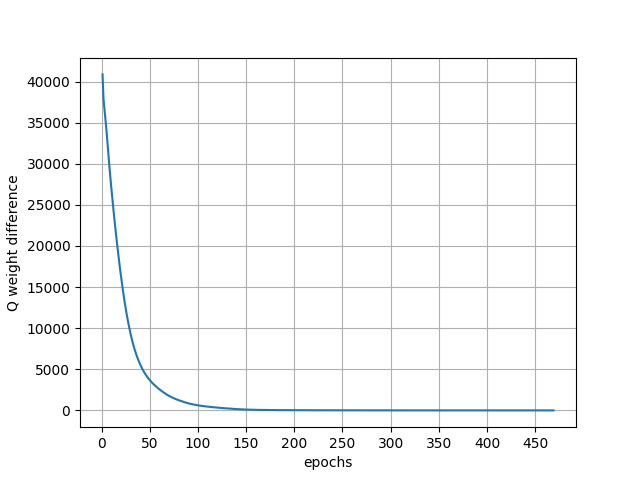
\includegraphics[scale=0.25]{./figure/QI_weight.png}
		\end{minipage}
	}%
\centering
\subfigure[200 最终结果]{
	\label{QI200}
	\begin{minipage}[t]{0.5\linewidth}
		\centering
		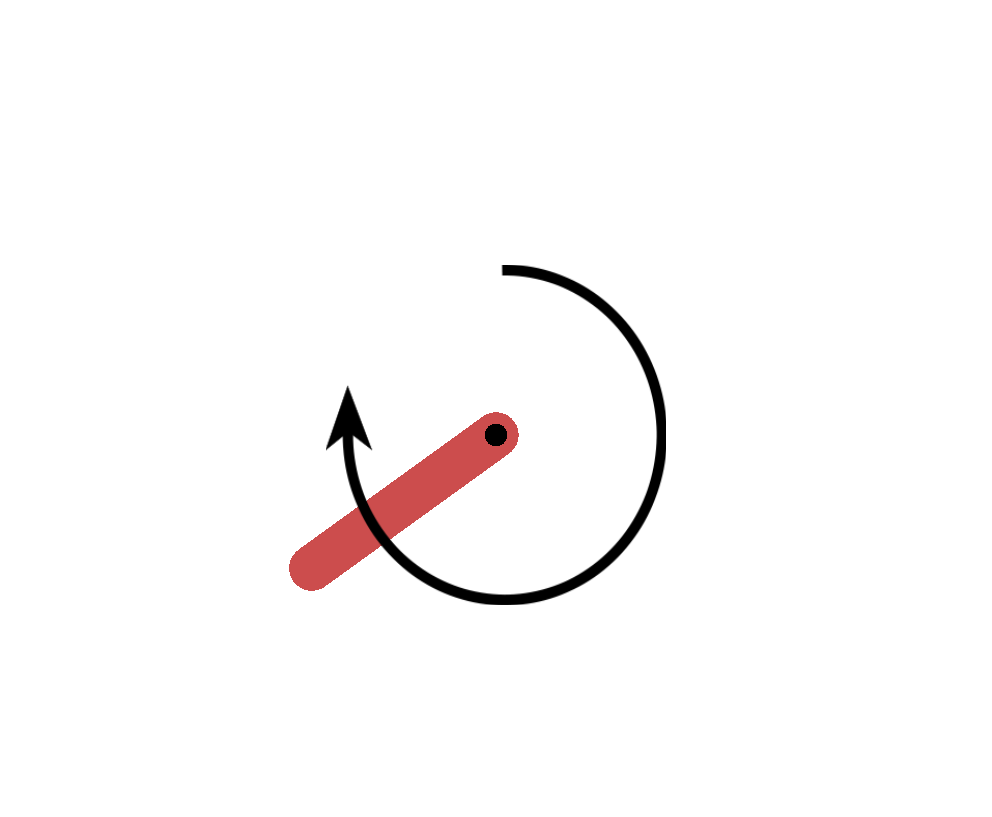
\includegraphics[scale=0.2]{./figure/QI-200.png}
	\end{minipage}
}%

		\centering
	\subfigure[300 Q函数权重变化]{
		\begin{minipage}[t]{0.5\linewidth}
			\centering
			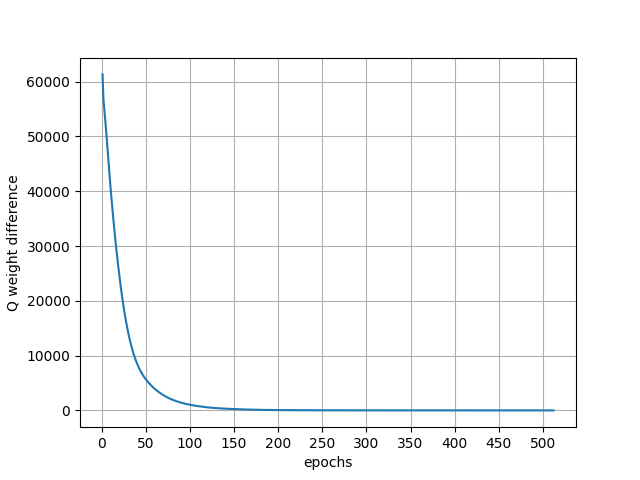
\includegraphics[scale=0.25]{./figure/QI_weight2.png}
		\end{minipage}
	}%
	\centering
	\subfigure[300 最终结果]{
		\label{QI300}
		\begin{minipage}[t]{0.5\linewidth}
			\centering
			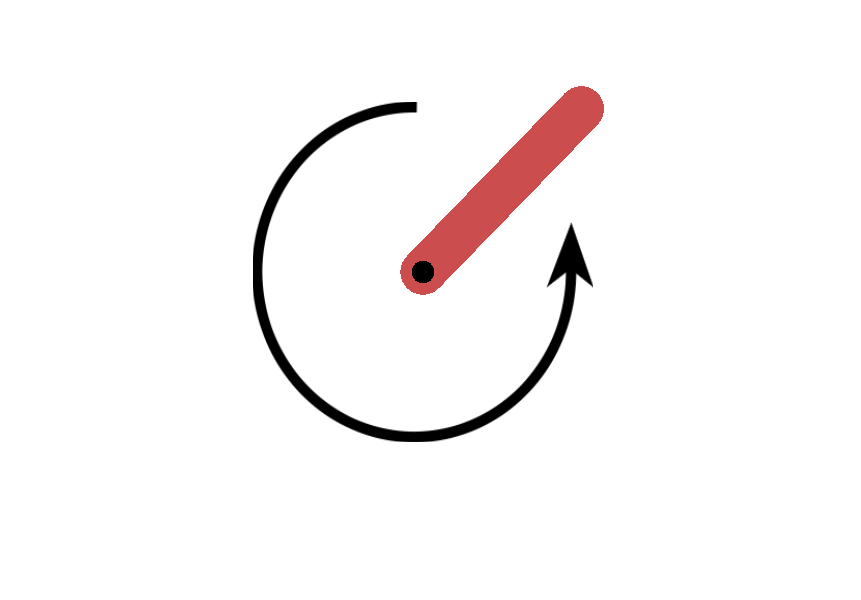
\includegraphics[scale=0.2]{./figure/QI-300.png}
		\end{minipage}
	}%

		\centering
\subfigure[500 Q函数权重变化]{
	\begin{minipage}[t]{0.5\linewidth}
		\centering
		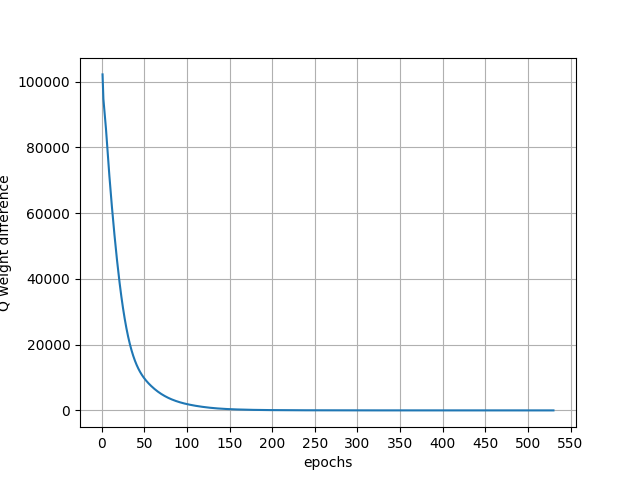
\includegraphics[scale=0.25]{./figure/QI_weight3.png}
	\end{minipage}
}%
\centering
\subfigure[500 最终结果]{
	\label{QI500}
	\begin{minipage}[t]{0.5\linewidth}
		\centering
		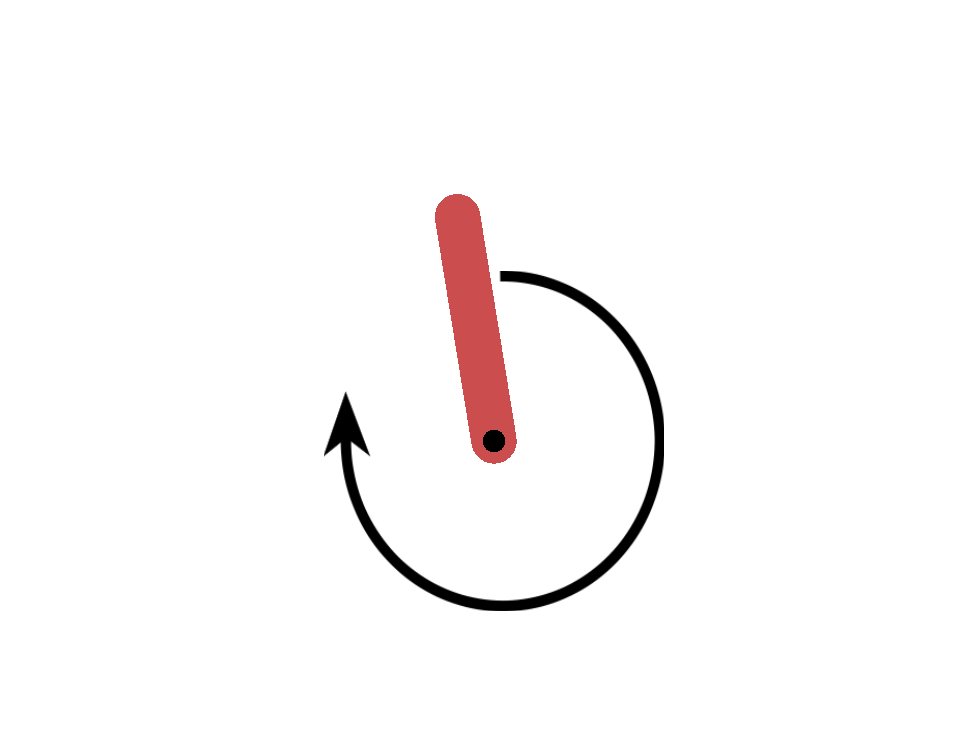
\includegraphics[scale=0.2]{./figure/QI-500.png}
	\end{minipage}
}%
\caption{离散Q价值迭代权重变化与迭代结果}
\label{QI}
\end{figure}

经过分析,我们认为产生问题的原因是空间离散太粗糙,并不能很好的刻画真实Q函数。为此我们进一步加细分割,将角度与角速度空间分别等距离分割 300 份,得到维度大小为 90000 的离散状态空间表示,重新进行训练。经过 512 步迭代,算法收敛。对获得的最优动作策略进行仿真模拟,我们发现摆杆仍然未达到目标位置,但是此刻摆杆已经在上半方震荡(图\ref{QI300}),相比于之前有了很大的提升。最后,我们进一步细分角度与角速度空间为500份,经过530次迭代算法收敛。对获得的最优动作策略进行仿真模拟,我们发现系统终于实现最优动作(图\ref{QI500})。三次实验的 Q 函数权重变化见图\ref{QI}。进一步,我们绘制出在三种离散空间中采取电压 -3V 动作的Q函数热力图(图\ref{QIheat})。可以发现分割越细致,Q函数变化越为平滑。
\begin{figure}[H]
	\centering
	\subfigure[200]{
		\begin{minipage}[t]{0.3\linewidth}
			\centering
			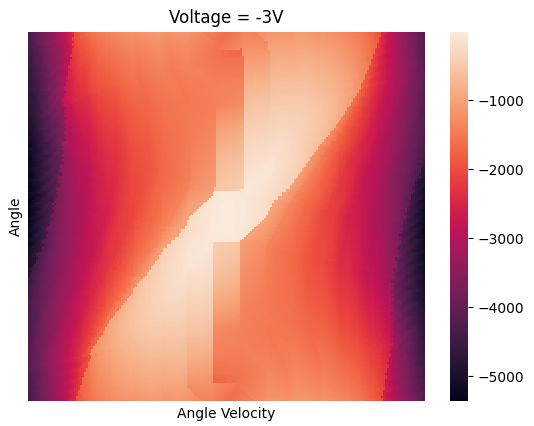
\includegraphics[scale=0.18]{./figure/QI200heat.png}
		\end{minipage}
	}%
	\centering
	\subfigure[300]{
		\begin{minipage}[t]{0.3\linewidth}
			\centering
			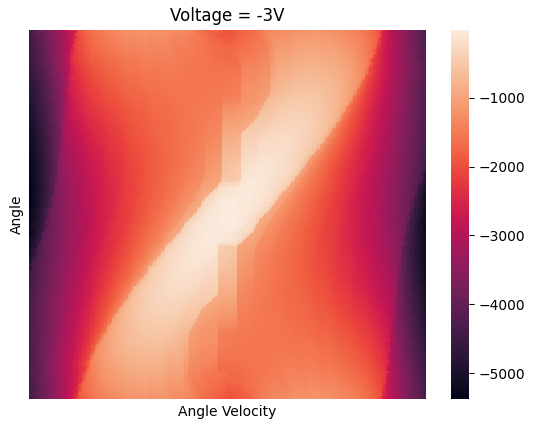
\includegraphics[scale=0.18]{./figure/QI300heat.png}
		\end{minipage}
	}%
	\centering
	\subfigure[500]{
		\begin{minipage}[t]{0.3\linewidth}
			\centering
			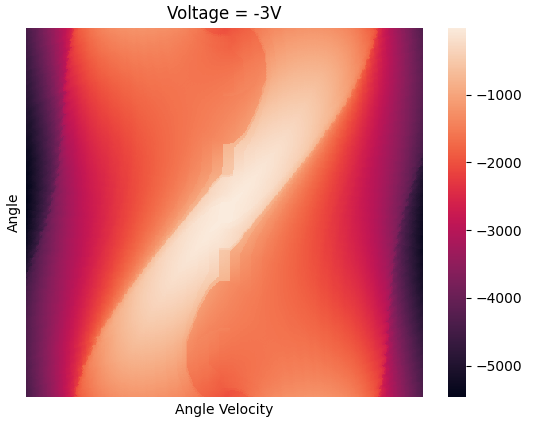
\includegraphics[scale=0.18]{./figure/QI500heat.png}
		\end{minipage}
	}%
\caption{离散Q价值迭代Q函数热力图}
\label{QIheat}
\end{figure}
 

\subsection{Sarsa算法}
我们尝试对于离散化状态空间使用Sarsa算法。我们将角度与角速度空间分别等距离分割 300 份,得到维度大小为 90000 的离散状态空间表示,对于每次迭代,我们采样10000次状态动作。500次迭代下,每幕的累计回报变化趋势可见图\ref{sarsa-reward}。

\begin{figure}[H]
	\centering
	\subfigure[Sarsa Reward 变化趋势]{
		\label{sarsa-reward}
		\begin{minipage}[t]{0.5\linewidth}
			\centering
			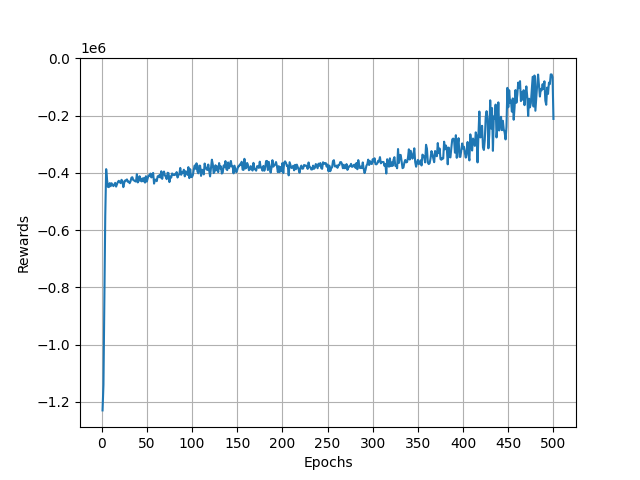
\includegraphics[scale=0.18]{./figure/DSarsa.png}
		\end{minipage}
	}%
	\centering
	\subfigure[Sarsa -3V下Q函数]{
		\begin{minipage}[t]{0.5\linewidth}
			\centering
			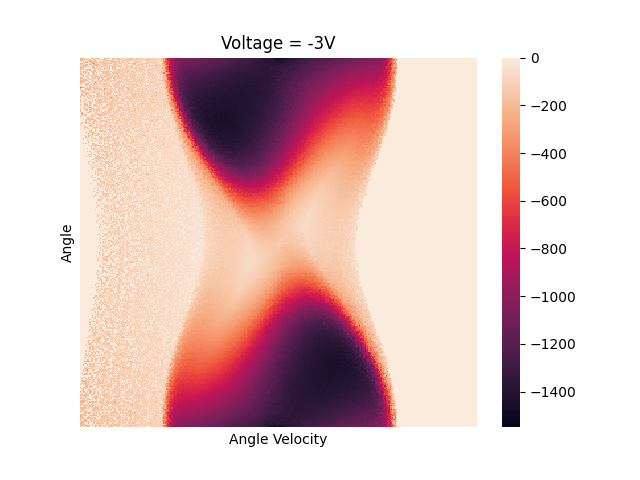
\includegraphics[scale=0.18]{./figure/sarsaheat.png}
		\end{minipage}
	}%
	
	\centering
	\subfigure[Sarsa($\lambda$) Reward 变化趋势]{
		\label{Sarsa-lam-reward}
		\begin{minipage}[t]{0.5\linewidth}
			\centering
			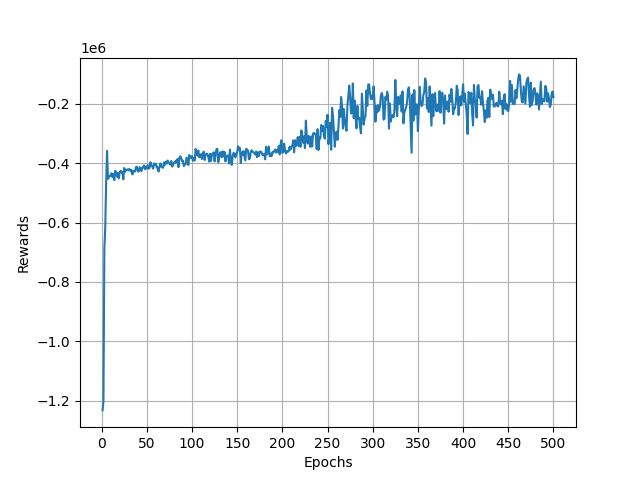
\includegraphics[scale=0.26]{./figure/DSarsa-lam.png}
		\end{minipage}
	}%
	\centering
	\subfigure[Sarsa($\lambda$) -3V下Q函数]{
		\begin{minipage}[t]{0.5\linewidth}
			\centering
			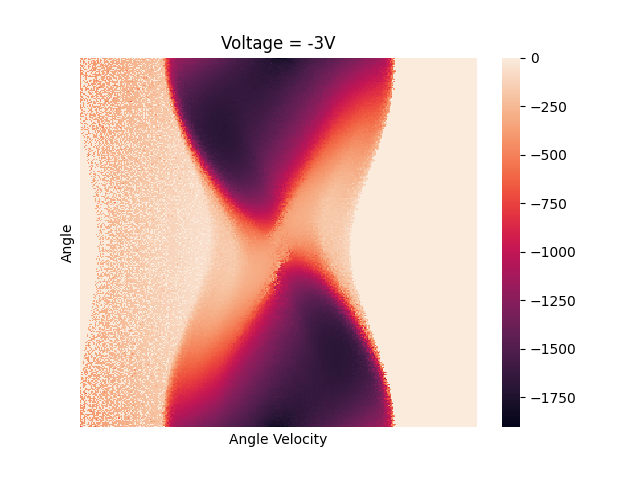
\includegraphics[scale=0.18]{./figure/Sarsalamheat.png}
		\end{minipage}
	}%
\caption{Sarsa算法累计回报变化与Q函数热力图}
\label{Sarsaheat}
\end{figure}

此外,我们引入资格迹,对 Sarsa 算法进行改进。同样的,我们将角度与角速度空间分别等距离分割 300 份,得到维度大小为 90000 的离散状态空间表示,对于每次迭代,我们采样10000次状态动作。500次迭代下,每幕的累计回报变化趋势可见图\ref{Sarsa-lam-reward}。

两种Sarsa算法均得到了最优控制,但通过比较累计回报变化趋势图,我们可以发现Sarsa算法大致在450步迭代时收敛,而使用资格迹的Sarsa$(\lambda)$ 算法在270步左右就获得收敛。在实际迭代过程中,由于每次迭代需要更新维护资格迹,计算时间并未太大提升。此外比较 Sarsa算法(图\ref{Sarsaheat})与离散Q价值迭代(图\ref{QIheat})同样在-3V动作下的Q函数,发现两者不太一样。进一步仔细观察可以发现,由于Sarsa算法基于采样得到,因此并未更新所有可能状态的Q值,这导致在热力图左右两侧出现大量的0值,而DP算法由于进行全局的搜索更新,因此会把很多无用状态的Q值也进行更新,由此可以进一步阐述基于采样算法效率更高的原因。

对于不同 $\lambda$ 下 Sarsa$(\lambda)$ 算法的表现我们也进行了相应的实验(图\ref{diff-lam})。可以发现 $\lambda=0.9$ 时,Sarsa$(\lambda)$算法累计回报的波动很小,但是在500步迭代中似乎并未收敛到最优控制,$\lambda=0.1$ 时, Sarsa$(\lambda)$ 仅通过250步左右迭代达到了最优控制,但之后整体的累计回报方差波动较大。
\begin{figure}[H]
	\centering
	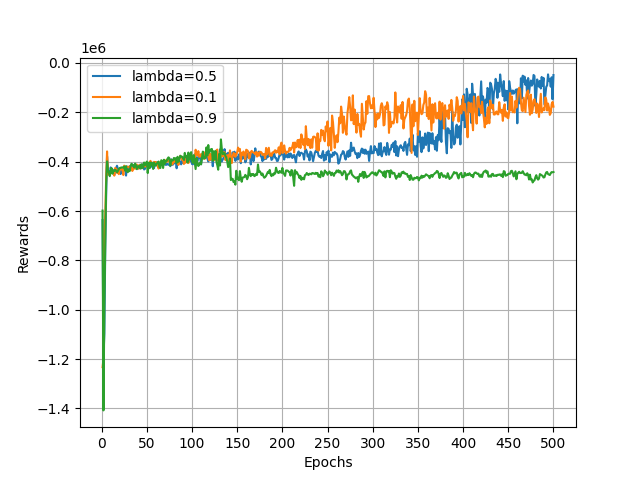
\includegraphics[scale=0.25]{./figure/diff-lam.png}
	\caption{不同$\lambda$下Sarsa($\lambda$) Reward 变化趋势}
	\label{diff-lam}
\end{figure}

\subsection{Q-Learning 算法}
对于 Q-Learning 算法,我们分别在离散化的状态空间和基于神经网络逼近器上进行训练。对于离散化的状态空间,我们将角度与角速度空间分别等距离分割 300 份,得到维度大小为 90000 的离散表示。对于逼近器方法,我们使用了一个隐藏层为128节点的单层神经网络,两者累计回报的变化趋势可见图\ref{QL-reward}、\ref{DQN-reward}。
\begin{figure}[H]
	\centering
	\subfigure[Q-Learning Reward 变化趋势]{
		\label{QL-reward}
		\begin{minipage}[t]{0.5\linewidth}
			\centering
			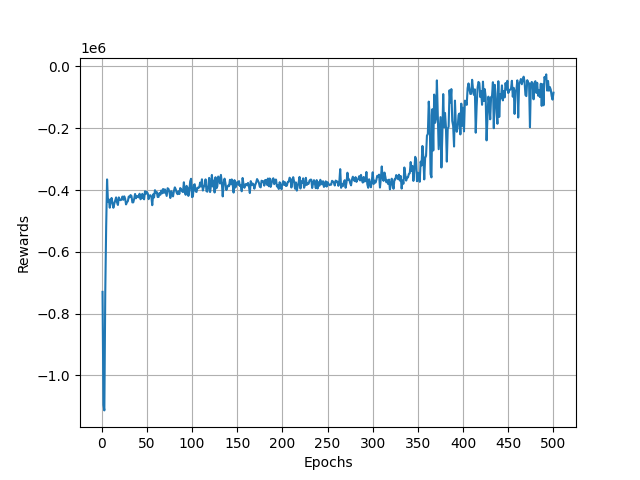
\includegraphics[scale=0.18]{./figure/DQL.png}
		\end{minipage}
	}%
	\centering
	\subfigure[Q-Learning -3V下Q函数]{
		\label{}
		\begin{minipage}[t]{0.5\linewidth}
			\centering
			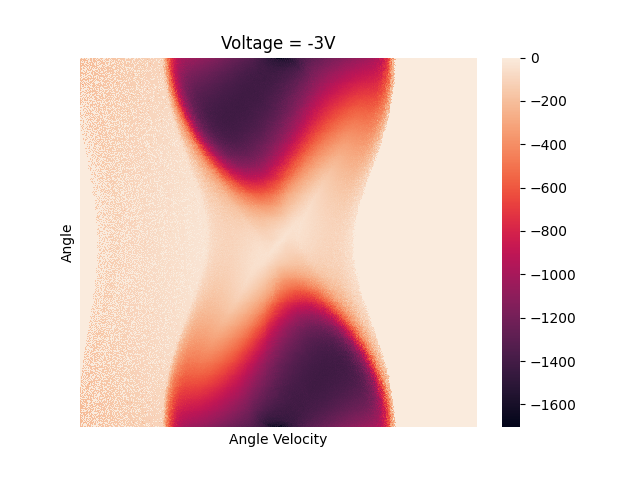
\includegraphics[scale=0.18]{./figure/Qlearningheat.png}
		\end{minipage}
	}%
	
	\centering
	\subfigure[DQN Reward 变化趋势]{
		\label{DQN-reward}
		\begin{minipage}[t]{0.5\linewidth}
			\centering
			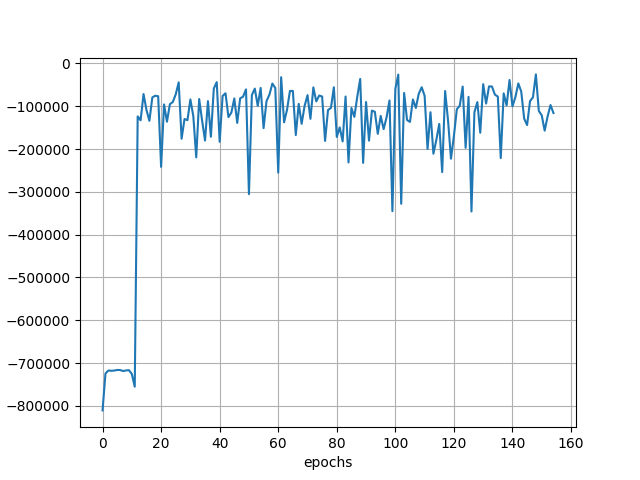
\includegraphics[scale=0.26]{./figure/DQN.png}
		\end{minipage}
	}%
	\centering
	\subfigure[DQN -3V下Q函数]{
		\label{}
		\begin{minipage}[t]{0.5\linewidth}
			\centering
			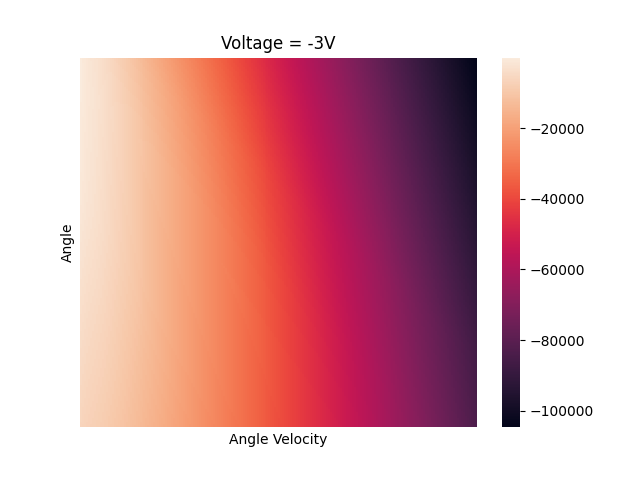
\includegraphics[scale=0.25]{./figure/DQNheat.png}
		\end{minipage}
	}%
	\caption{Sarsa算法累计回报变化与Q函数热力图}
	\label{DQNheat}
\end{figure}
从图中可以发现,DQN算法在20步左右迭代时已经收敛,显示出神经网络逼近器的强大。但是同时在实验中发现,神经网络逼近器并不稳定,在大量训练下会出现过拟合而落入摆杆停止在初始位置不摆动的情形。且由热力图可以发现,神经网络逼近器求出的-3V电压下的Q函数与其他方法求出的并不相同。

\subsection{失败的实验算法}
除去代码本身存在一定逻辑错误的原因外,我们对失败实验算法出现的情况进行一定的理论分析。
\subsubsection{基于RBF核的线性逼近器+Sarsa算法}
我们从角度空间和角速度空间分别等距离取了10个点,并两两组合为中心构造了100个RBF核函数作为状态空间的特征提取器,其中RBF核的协方差矩阵取为固定对角阵,对角元素为角度空间和角速度空间两个点间的取值距离。我们尝试使用了 LSPI 和随机梯度下降+Sarsa的方法对线性逼近器进行梯度更新,但均为获得最优控制。对状态空间采样,画出固定-3V电压下的Q函数(图\ref{RBF})。可以发现,虽然已经过了500轮的迭代,除了在 初始状态小范围内,似乎Q函数并未得到有效更新。另一方面,在训练过程中发现在初始状态小范围内,三个动作的价值函数很接近,以至于初始情况经常会在三个动作选择上震荡。
\subsubsection{基于策略梯度的强化学习算法}
我们尝试了REINFORCE 算法与 Advantage Actor-Critic 算法,但结果并未收敛到最优控制,收敛结果与200*200离散空间的离散Q价值迭代算法类似。基于此我们分析可能有两种原因导致此结果,一是价值函数设置的不合理。可以发现在奖励函数的设置中,对于大角速度的惩罚是很严重的,此外对于电压的惩罚会进一步加重对角速度的惩罚,进而影响倒立摆并不愿意摆起。另一方面,考虑到与DQN算法实验类似的情况,神经网络的拟合存在过拟合,且不稳定的情况,而基于策略梯度的强化学习算法容易落入局部最优解中,从而无法实现全局最优。

对于第一种情况,我们实验并提供了一种可能的解决思路。考虑到倒立摆系统首要目标是将其摆到最高点,模仿Actor-Critic的思想,我们可以先加大奖励函数中对角度的惩罚,使得倒立摆能够摆起至最高点,此时采样包含更多目标奖励的信息。最后,再还原奖励函数至默认形式,重新进行一轮训练。我们对此进行实验,效果有所改善但并未成功。
\begin{figure}
	\centering
	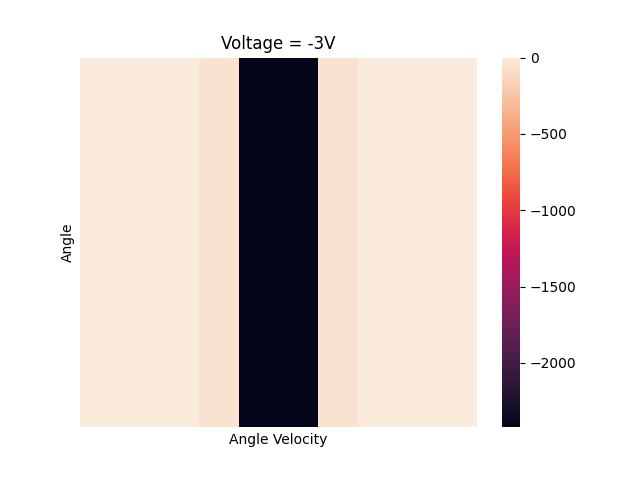
\includegraphics[scale=0.25]{figure/sarsa_lam_linear.png}
	\caption{RBF核线性逼近器+Sarsa($\lambda$) Q函数}
	\label{RBF}
\end{figure}
\subsection{实验代码}
我们已将代码上传至\href{https://github.com/Kingsley-Cheng/UCAS/tree/main/ReinforcementLearning/Homework1}{Github 仓库},希望可以对已实现的代码进行进一步并行计算等方面的改进和优化,对失败的代码进行检测与修正,并通过分支进行提交。


\section{总结}
\subsection{倒立摆系统}
在实验过程中,我们经常发现倒立摆存在如下几种局部最优情况:
\begin{itemize}
\item 停止在初始状态不做动作;
\item 倒立摆直接加速到最大速度,摆到水平位置左右后不断加电压使其平衡,而没有学会能量的累积;
\item 倒立摆突破水平位置的限制,但角速度过大,导致倒立摆不断的打转,直流电机并未因此而加反向电压进行控制。
\end{itemize}
出现这些情况的原因十分复杂,我们并未对此进行深入分析。
\subsection{强化学习各方法}
通过实验,我们对强化学习各算法有如下几点认识:
\begin{itemize}
\item 基于离散状态空间的算法在该问题上显得更为稳定,基于逼近器的方法则较为敏感。
\item 基于全局的离散Q价值迭代训练效率很慢,更新了大量没有意义的状态Q价值函数。基于采样的强化学习方法效率更高,但受采样随机性影响,存在一定波动性。
\item 基于资格迹的Sarsa$(\lambda)$算法中,$\lambda$值的大小决定了算法的收敛性与稳定性。$\lambda$ 值越大收敛越慢,但波动更小。
\item 同样基于采样的强化学习算法方面,由于采用离策略,Q-Learning 算法的累积回报价值会显得更高。而Sarsa因为存在随机探索性,动作更为保守。
\item DQN学习到的Q价值函数与离散状态空间下学到的Q价值函数并不相同。
\end{itemize}
\section*{Acknowledgment}
部分代码(主要Rendering方面)参考了\href{https://github.com/dalek-who/Inverted-Pendulum}{dalek-who在Github中的部分代码},再次表示感谢。

\section*{References}

\begin{thebibliography}{00}
\bibitem{b1} Sutton R S, Barto A G. Reinforcement learning: An introduction[M]. MIT press, 2018.
\bibitem{b2} 张伟楠,动手学强化学习. (2022). 中国: 人民邮电出版社.
\end{thebibliography}

\end{document}
